\documentclass[a4paper]{memoir}

\usepackage[a4paper,margin=2cm]{geometry}
\usepackage[utf8]{inputenc}
\usepackage{times}
\usepackage[english]{babel}
\usepackage{multirow}
\usepackage{amsmath,graphicx}
\usepackage{hyperref}
\usepackage{fancyvrb}
\usepackage[textwidth=2.5cm, textsize=small]{todonotes}

\usepackage{xspace}
\newcommand{\vonda}{VOnDA\xspace}

\pgfdeclareimage[width=.99\columnwidth]{vondagui}{VondaGui}

\begin{document}

\title{\vonda, A Framework for Dialogue Management}
\author{Bernd Kiefer, Anna Welker}
\date{\today}

\maketitle

\tableofcontents

\chapter{Purpose}

\vonda is a framework to implement the dialogue management functionality in
dialogue systems. Although domain-independent, \vonda is tailored towards
dialogue systems with a focus on social communication, which implies the need
of a long-term memory and high user adaptivity. \vonda's specification and
memory layer relies upon (extended) RDF/OWL, which provides a universal and
uniform representation, and facilitates interoperability with external data
sources.

\vonda consists of three parts: A programming language tailored towards the
specification of reactive rules and transparent RDF data store usage, a
compiler that turns source code in this language into Java code, and a run-time
core, that supports implementing dialogue management modules using the compiled
rules.

The framework is domain-independent, it was originally designed to for
multi-modal human-robot interaction, but there is currently no \emph{special}
functionality in the core to either support the multi-modality nor the
human-robot interaction. The architecture of the framework is open and powerful
enough to add these things easily.

\chapter{Sketching a Simple Interaction Manager}

The simplest version of an interaction manager analyses natural language
coming from the user, and generates natural language and gestures for the robot
resp. its virtual replacement, the avatar. Generation is based on incoming
stimuli, like speech or text input, or high-level action requests coming from
some strategic planning component, or any other sensor input, if available.

The interaction manager will get several input types from the nexus, the ones
currently foreseen are: input from automatic speech recognition (ASR) or typed
natural input, user parameters, like name, age, hobbies, etc. but also more
dynamic ones like mood or health data, and also triggers from high-level
planning.

All these inputs are stored as RDF data, based on an ontology developed as part
of the interaction manager, and available to all other components as a data
format specification.

When new data is added, a set of declaratively specified reactive rules will
propose dialogue moves or other actions and send these proposals to the action
selection mechanism. The selection mechanism selects the ``best'' of the
proposed actions and sends it back. If the proposed action results in dialogue
acts, these are turned into verbal output and gestures with the help of a
multimodal generation component, which retrieves parameters from the RDF
database to adapt the generation to the user's likings, and can also take into
account sensory data such as her or his estimated mood.

\section{Internal structure}

As shown in the picture below, the interaction manager consists of the RDF
store, which also contains the functionality to store incoming data in the
format specified by the ontology, thereby making it readily accessible for
other components.

The second major component is the rule processor for the dialogue management
rules, which generates proposals for actions when new incoming data
arrives. The rules not only use the new data, but also the interaction history
stored in the RDF database to take its decisions.

The last two parts are a robust natural language interpretation module (not
explicitly shown in the picture), which turns spoken or written utterances
into dialogue acts, possibly with an intermediate step that involves a more
elaborate semantic format, and a multimodal generation component, which turns
outgoing dialogue acts into natural language utterances and gestures.

\vspace*{4ex}

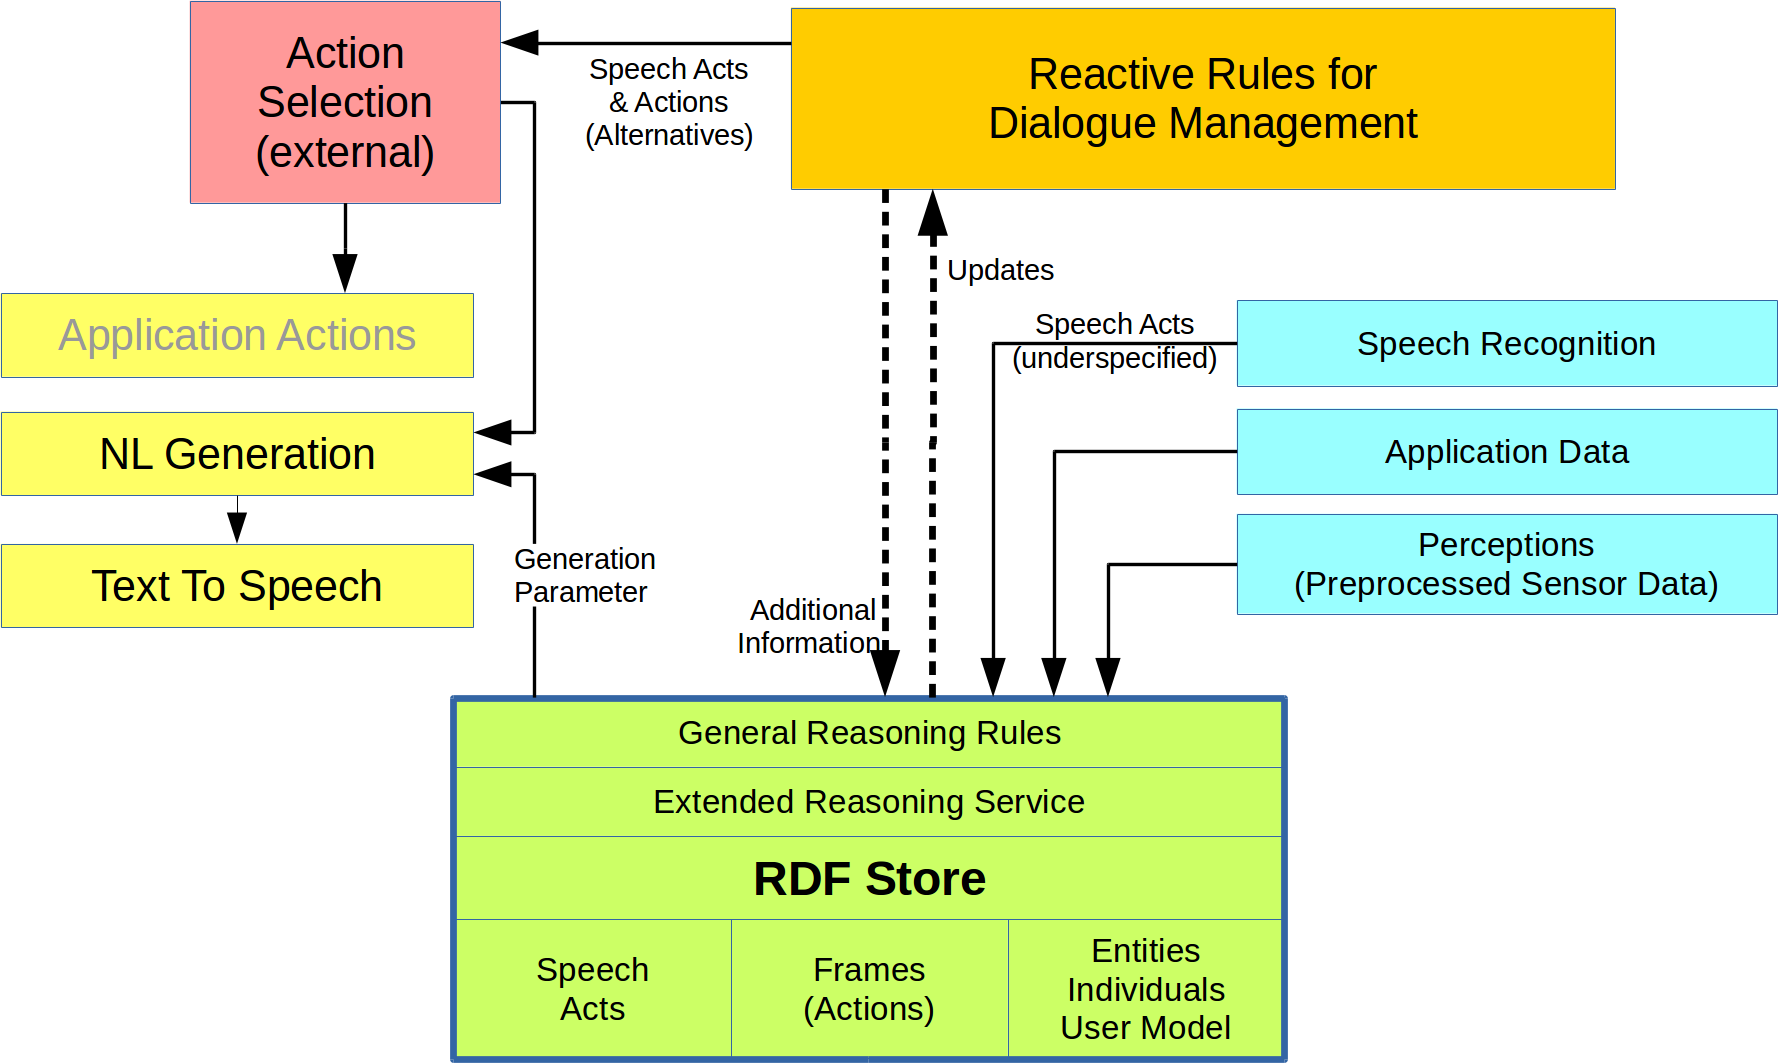
\includegraphics[width=.9\textwidth]{rudimant.png}

%\section{Options for translating rules and .rudi files}

Naming convention: a label followed by a colon followed by an \emph{if} is
called \emph{rule} from now on.

There are two main options to translate:
\begin{itemize}
\item[A)] translate the whole project into one large Java class / method
  Problems with this approach
  \begin{itemize}
  \item The relation to the source code is hard to track: no modularity, one
    large blob
  \item The execution regime can not be changed except by changing the
    translation (no dynamic adaptation of execution)
  \end{itemize}
\item[B)] Create a class for each .rudi file and each top-level rule
  \begin{itemize}
  \item Clear structure that is isomorphic to the .rudi files
  \item Dynamic execution strategy is easier to imagine, albeit not really
    feasible (do we want/need it?)
  \item Variables on the top level of a file can be implemented by class
    fields and fully specified access, such as Introduction.special\_variable
  \end{itemize}
\end{itemize}

We're going for version B), assuming that most of the variables which have
non-local scope are state variables in the agent, which also might be
specified in special top-level files. These should also contain specifications
for general framework functions, i.e., the whole signatures including types
for the arguments and return types, to enable advanced type checking.

Similar files could be used for custom user state variables and functions,
i.e., for Quiz logic, custom knowledge bases, etc.

Embedded rules will be treated differently to avoid the overhead of handling
local scope and lifetime of variables.

\texttt{return} statements can have optional labels that indicate the exit
point / level, which may be local rule, top-level rule or file. A return
without label exits from the innermost scope.

Example for a top-level rule:

\begin{verbatim}
a:
if ( XXXX ) {
  x = child_27;
  b:
  if (YYYY) {
     x = child_3;
     c:
     if ( ZZZZ ) {
        ....
        if (....) return b:;
        ....
     } // c: ends
     ....
  } // b: ends
} // a: ends
\end{verbatim}

The labeled exits are implemented by setting flags in a bit mask that are
tested in the following to skip code not to be executed:
\newpage
Possible translation, (example starts at \texttt{return b:})
\begin{verbatim}
a:
if ( XXXX ) {
  x = child_27;
  b:
  if (YYYY) {
     x = child_3;
     c:
     if ( ZZZZ ) {
        ....
        if (....) {
           // return b:;
           returnMask |= b_mask;
        }
        if ((returnMask | (a_mask | b_mask | c_mask)) == 0) {
           ....
        }
     } // c: ends
     if ((returnMask | (a_mask | b_mask)) == 0) {
     ....
     }
  } // b: ends
  if ((returnMask | a_mask) == 0) {
  }
} // a: ends
\end{verbatim}

\section{Writing to Rudi (with care)}
If you are in a state where you want to immediately stop processing and leave all
rules, use a call to the method Agent.stopProcessing() to jump out of the topmost
rule file.

%%% Local Variables:
%%% mode: latex
%%% TeX-master: "master"
%%% End:


\chapter{Auspacken, Installation, Starten}

\section{The RDF Database HFC} \label{sec:hfc}

\vonda follows the information state/update paradigm. The information state is
realized by an RDF store and reasoner with special capabilities
(HFC \cite{krieger2013efficient}), namely the
possibility to directly use $n$-tuples instead of triples. This allows to
attach temporal information to every data chunk \cite{Krieger:FOIS2012,
  krieger2014detailed}. In this way, the RDF store can represent \emph{dynamic
  objects}, using either \emph{transaction time} or \emph{valid time}
attachments, and as a side effect obtain a complete history of all changes.
HFC is very efficient in terms of processing speed and memory footprint, and
has recently been extended with stream reasoning facilities. \vonda can use HFC
\todo{AW: Just asking: How long can we still talk of ''recently extended''?}
either directly as a library or as a remote server, also allowing for more
than one instance if needed (for this feature see section \ref{sec:2ndHfc}).

The following is the syntax of HFC queries (EBNF):
\begin{table}[htbp]
  \centering\small
\begin{verbatim}
<query>     ::= <select> <where> [<filter>] [<aggregate>] | ASK <groundtuple>
<select>    ::= {"SELECT" | "SELECTALL"} ["DISTINCT"] {"*" | <var>^+}
<var>       ::= "?"{a-zA-Z0-9}^+ | "?_"
<nwchar>    ::= any NON-whitespace character
<where>     ::= "WHERE" <tuple> {"&" <tuple>}^*
<tuple>     ::= <literal>^+
<gtuple>    ::= <constant>^+
<literal>   ::= <var> | <constant>
<constant>  ::= <uri> | <atom>
<uri>       ::= "<" <nwchar>^+ ">"
<atom>      ::= "\""  <char>^* "\"" [ "@" <langtag> | "^^" <xsdtype> ]
<char>      ::= any character, incl. whitespaces, numbers, even '\"'
<langtag>   ::= "de" | "en" | ...
<xsdtype>   ::= "<xsd:int>" | "<xsd:long>" | "<xsd:float>" | "<xsd:double>" |
                "<xsd:dateTime>" | "<xsd:string>" | "<xsd:boolean>" | "<xsd:date>" |
                "<xsd:gYear>" | "<xsd:gMonthDay>" | "<xsd:gDay>" | "<xsd:gMonth>" |
                "<xsd:gYearMonth>" | "<xsd:duration>" | "<xsd:anyURI>" | ...
<filter>    ::= "FILTER" <constr> {"&" <constr>}^*
<constr>    ::= <ineq> | <predcall>
<ineq>      ::= <var> "!=" <literal>
<predcall>  ::= <predicate> <literal>^*
<predicate> ::= <nwchar>^+
<aggregate> ::= "AGGREGATE" <funcall> {"&" <funcall>}^*
<funcall>   ::= <var>^+ "=" <function> <literal>^*
<function>  ::= <nwchar>^+
\end{verbatim}
  \caption{BNF of the database query language}
  \label{tab:hfcquerybnf}
\end{table}

%\paragraph{Notes}

The reserved symbols \texttt{ASK}, \texttt{SELECT}, \texttt{SELECTALL},
\texttt{DISTINCT}, \texttt{WHERE}, \texttt{FILTER} and \texttt{AGGREGATE}
do \emph{not} need to be written in uppercase, but neither \texttt{filter} predicates nor \texttt{aggregate} functions should be named like reserved symbols.

\emph{don't-care} variables should be marked \emph{explicitely} by using
\verb|?_|, particularly if \texttt{SELECT} is used with \verb|*| as in:
\begin{verbatim}
     SELECT DISTINCT * WHERE ?s <rdf:type> ?_
     SELECT * WHERE ?s <rdf:type> ?o ?_
\end{verbatim}
To change the object position without projecting it you can use \emph{don't-care} variables:
\todo{AW: I do have an idea of how to write hfc queries of the simplicity that is sufficient for most DM stuff, and I have no understanding of what this means... Explain?}
\begin{verbatim}
     SELECT ?s WHERE ?s <rdf:type> ?o ?_ FILTER ?o != <foo-class>
\end{verbatim}

Aggregates in HFC take whole tables or parts of them and calculate a result based on their entities. As the type of aggregates and filter functions cannot be overloaded, there are multiple similar functions for different types, e.g. F for \texttt{float}, L for \texttt{long}, D for \texttt{double}, I
for \texttt{int}, and S for \texttt{String}.

\begin{table}[htbp]
  \centering
 \begin{tabular}{lll}
   CountDistinct&  FSum&             LMax\\
   Count&          FMean&            LMean\\
   DMean&          LGetFirst2&       LMin\\
   DSum&           LGetLatest2&      LSum\\
   DTMax&          LGetLatest&       LGetLatestValues\\
   DTMin&          LGetTimestamped2& Identity     \\
 \end{tabular}
  \caption{Available aggregates}
  \label{tab:hfcaggregates}
\end{table}

Apart from \verb|==| and \verb|!=|, functional operators can be used in \texttt{filter} expressions as well. As for aggregates, there are multiple versions of the same function for different data types.

\begin{table}[htbp]
  \centering\small
\begin{tabular}{llll}
CardinalityNotEqual &        FNotEqual &               IntStringToBoolean &      LMin \\
Concatenate &                FProduct &                IProduct &                LNotEqual \\
DTIntersectionNotEmpty &     FQuotient &               IQuotient &               LProduct \\
DTLessEqual &                FSum &                    IsAtom &                  LQuotient \\
DTLess &                     GetDateTime &             IsBlankNode &             LSum \\
DTMax2 &                     GetLongTime &             IsNotSubtypeOf &          LValidInBetween\\
DTMin2 &                     HasLanguageTag &          ISum &                    MakeBlankNode \\
EquivalentClassAction &      IDecrement &              IsUri &                   MakeUri \\
EquivalentClassTest &        IDifference &             LDecrement &              NoSubClassOf \\
EquivalentPropertyAction &   IEqual &                  LDifference &             NoValue \\
EquivalentPropertyTest &     IGreaterEqual &           LEqual &                  PrintContent \\
FDecrement &                 IGreater &                LGreaterEqual &           PrintFalse \\
FDifference &                IIncrement &              LGreater &                PrintSize \\
FEqual &                     IIntersectionNotEmpty &   LIncrement &              PrintTrue \\
FGreaterEqual &              ILessEqual &              LIntersectionNotEmpty &   SameAsAction \\
FGreater &                   ILess &                   LIsValid &                SameAsTest \\
FIncrement &                 IMax2 &                   LLessEqual &              SContains.java\\
FLessEqual &                 IMax &                    LLess &                   UDTLess \\
FLess &                      IMin2 &                   LMax2 \\
FMax &                       IMin &                    LMax \\
FMin &                       INotEqual &               LMin2 \\
\end{tabular}
\caption{Available filter functions}
  \label{tab:hfcfunctions}
\end{table}

\subsection{Usage of HFC in \vonda} \label{sec:hfc_usage}

The RDF store contains the dynamic and the terminological knowledge:
specifications for the data objects and their properties, as well as a
hierarchy of  dialogue acts,  semantic frames and their arguments. These
specifications are also used by the compiler to infer the types for property
values (see sections \ref{sec:typeinference} and \ref{sec:rdfaccesses}), and form a declarative API to
connect new components, e.g., for sensor or application data.

The ontology contains the definitions of dialogue acts, semantic frames, class
and property specifications for the data objects of the application, and other
assertional knowledge, such as specifications for ``forgetting'', which could
be modeled in an orthogonal class hierarchy, and supported by custom deletion
rules in the reasoner.

For queries which are too complex to be handled the \vonda way, or if you want to do reasoning which for efficiency reasons should be handled by HFC rather than Java (e.g., if you are filtering for specific property values in a pool of many instances of the same class), there also is a direct communication port to HFC.

\begin{lstlisting} [language=Java]
List<String> uris = new ArrayList<>();
// the ancestor is that hyponym which has the shortest path to syn
String ancestors = "select ?s  where ?s <wn20schema:hyponym> {} ?_ ";
QueryResult qr = proxy.selectQuery(ancestors, syn);
uris = RdfProxy.getValues(qr);
\end{lstlisting}

The above code, for example, retrieves all hyponyms of a given synset \texttt{syn}.

Currently, it is recommended to place such code in Java methods that you can then use in your \vonda code to indirectly perform the queries. In the future, functionality will be added to support facilitated query construction directly in \vonda code.


\section{Rudimant-Kompiler und Laufzeitsystem}

Der Rudimant-Kompiler übersetzt Regeldateien mit Extension \texttt{.rudi} in
Java-Dateien. Dazu braucht er eine Ontologie, in der die RDF Klassen und
Prädikate, die im \texttt{.rudi}-Code verwandt werden, spezifiziert sind.

Im Fall des POC liegen die Quelldateien in \texttt{src/main/rudi} und die
dazugehörende Ontologie in \texttt{src/main/resources/ontology}. Damit HFC
die Ontologie benutzen kann, muss sie im ntriples-Format vorliegen. Die
derzeitige Ontologie wird mit Protégé erstellt und aus dem OWL-XML Format
mit Hilfe des \texttt{rapper}-Tools in eine \texttt{.nt} ntriples Datei
übersetzt. \texttt{rapper} ist Teil des Ubuntu-Package \texttt{raptor2-utils},
das Script \texttt{ntcreate} im \texttt{poc} Verzeichnis updated alle nicht
aktuellen \texttt{.nt} Files aus den \texttt{.owl} Versionen.

Weitere settings, die für die Kompilation wichtig sind, finden sich in der
Datei \texttt{herbea.yml}, die von \texttt{compile} Skript benutzt wird. Auch
hier sind alle relativen Pfade relativ zum Verzeichnis, in dem die
\texttt{.yml} Datei liegt.

Für standalone Mockup-Tests kann der POC auch isoliert mit dem \texttt{run.sh}
script gestartet werden, die ``Sensordaten'' werden dann nach und nach in
der main-Methode eingespielt.

Der folgende Text ist leider unvollständig und muss noch ergänzt werden. Für
die meisten Konstrukte gibt es einige Beispiele in den \texttt{rudi}
Quelldateien.

\subsection{Rudimant Regeln}

%{\Huge TODO: testen, ob alle Beispiele so funktionieren, wie sie sollen !!!!!!}

\subsubsection{''Globale'' Funktionen und Variablen}

Für Funktionen, die nicht oder nur umständlich in rudi-Code implementiert werden können, sollte der Nutzer eine Javaklasse MyAgent von der abstrakten Klasse Agent ableiten. Funktionen und Variablen, die in dieser Klasse deklariert wurden und später im rudi-Code benutzt werden sollen, müssen mit vollständiger Typangabe in einer Datei MyAgent.rudi registriert werden, sodass die Typinferenz von rudimant sie korrekt berücksichtigen kann (zur Syntax siehe \ref{rudimant-Typinferenz}).\\
Die Klasse MyAgent mitsamt Packagenamen muss in der config.yml Datei eines Projektes unter dem Eintrag ''wrapperClass'' spezifiziert werden, um im Compile-Schritt einen Effekt zu zeigen. Rudimant nutzt die Klasse MyAgent dann als Superklasse der im Compile-Schritt angegebenen Datei im rudi-Format und verlinkt Funktionsaufrufe und Variablennutzungen in allen untergeordneten rudi-Dateien auf diese, sodass korrekte Aufrufe im resultierenden Java-Code gewährleistet sind.

\subsubsection{RDF Zugriff, funktionale vs. relationale Prädikate
  \texttt{+=}, \texttt{-=}}

\begin{minipage}{0.4\textwidth}
\begin{verbatim}
Child c;
String name = c.name;
c.name = "new name";
\end{verbatim}
\end{minipage}
\begin{minipage}{0.6\textwidth}
\begin{verbatim}
String name = (String)c.getValue("<upper:name>");
c.setValue("<upper:name>", "new name");
\end{verbatim}
\end{minipage}
\newline
Durch die Verbindung zu hfc während des Compile-Vorganges hat rudimant vollen Zugriff auf die Datenbank und kann nicht nur Rdf-Objekte anhand ihrer Typen erkennen, sondern auch erkennen, wann ein Feldzugriff auf ein Rdf-Objekt erfolgt und ihn in solchen Fällen in einen Zugriff auf die Datenbank umwandeln. Dies ist sowohl für Zugriffe auf Properties als auch für Änderungen ihres Inhalts möglich und lässt sich, sofern dies in der verwendeten Ontologie möglich ist, beliebig oft hintereinander ausführen.\\

TODO: funktional vs relational?

Die beiden Operatoren \texttt{+=} und \texttt{-=} sind in rudimant überladen. Sie können sowohl wie in Java zum Rechnen mit Integer, float und double verwendet werden, als auch im Zusammenspiel mit Sets und Listen. $ a += b $ wird hierbei in $ a.add(b) $ umgewandelt, $ a-= b $ resultiert in $ a.remove(b) $.
  
\subsubsection{Regeln und Labels}

\begin{verbatim}
introduction:
  if (introduction){
    if (user.unknown){
      ask_for_name:
        if (talkative) {
          askForName();
        }
    } else {
      greetUser();
    }
  }
\end{verbatim}

Das Kernstück von rudimant sind die Dialogregeln. Eine Regel beginnt mit ihrem Namen, einem möglichst aussagekräftigen Label, gefolgt von einem Doppelpunkt. Anschließend folgt ein if-statement. Die Clause des Statements drückt die Bedingung aus, unter der die Regel ausgeführt werden soll, im Body steht der auszuführende Code.\\
Aussagekräftige Labels sind zum Debugging wichtig. Der generierte Code kann zur Laufzeit debuggt werden, indem man in Agent den Flag ... setzt. Der Output des Loggers wird dann das Label jeder Regel, die evaluiert wird, zusammen mit der Auswertung der Bedingung angeben.\\
% Bsp debugging-output
Regeln können beliebig tief geschachtelt werden, d.h., jede Regel kann wiederum Subregeln in ihrem Body haben.

%\subsubsection{Propose}

\subsubsection{Struktur einer Datei im rudi-Format}

Anders als Java stellt rudimant nicht den Anspruch, dass die Einträge in einer Datei in irgendeine Form von übergeordneter Struktur gefasst werden. Die Regeln können ebenso wie Funktionsdeklarationen direkt in die Datei geschrieben werden. Dasselbe gilt für jede Art valider (Java-) Statements, wie etwa Zuweisungen, for-Schleifen usw.. Rudimant wird bei der Kompilation eine Java-Klasse erstellen, in die es die Funktionen sowie die Regeln, zu Funktionen transformiert, einträgt. Alle weiteren Statements werden in der korrekten Reihenfolge in die erzeugte Methode process() verschoben, wobei generierte Aufrufe an die Regelfunktionen zwischen ihnen gewährleisten, dass die Regeln und Statements in der Reihenfolge ausgeführt werden, die im rudi-Code spezifiziert war. Dies ermöglicht also, nicht in Regeln gefasste Abbruchbedingungen einzubauen, unter denen die Ausführung der ganzen Datei - und möglicher importierter Dateien - sofort beendet werden soll.\\
Auf diese Art deklarierte Variablen werden als Klassenvariablen angelegt.

\subsubsection{Dialogakte und Hütchen} \ {\Large\verb|^|}

\begin{verbatim}
emitDA(#Inform(Answer, what=^solution));
\end{verbatim}

\subsubsection{Typinferenz} \label{rudimant-Typinferenz}

Rudimant erlaubt statische Typzuweisungen sowie Casting, beides ist jedoch nicht zwingend notwendig.\\
Ist beispielsweise der Typ der rechten Seite einer Variablendeklaration mit Zuweisung bekannt oder inferierbar, so ist es nicht notwendig, den Typ der Variablen explizit anzugeben.\\
Als zeitsparendes Feature bietet rudimant insbesondere das automatische Vervollständingen von bool'schen Ausdrücken in den Clauses von if, while und for an. Da in diesem Fall bekannt ist, dass das Ergebnis boolean sein muss, ergänzt rudimant automatisch den Test auf die Existenz eines Objektes in der Clause, sollte dieses nicht Typ boolean sein. Bei Feldzugriffen testet es für jeden Teilzugriff, dass das erhaltene Objekt nicht null ist, um einer NullPointerException zur Laufzeit des generierten Codes vorzubeugen.

\subsubsection{Überladene Vergleichsoperatoren und Tests}

\begin{minipage}{0.4\textwidth}
\begin{verbatim}
if (speechAct <= #Question){
  ...
}
\end{verbatim}
\end{minipage}
\begin{minipage}{0.6\textwidth}
\begin{verbatim}
if (isSmallerEqual(speechAct, new DialogueAct("Question")) {
  ...
}
\end{verbatim}
\end{minipage}
\newline


\begin{minipage}{0.4\textwidth}
\begin{verbatim}
if (! c.user.personality.nonchalance){
  ...
}
\end{verbatim}
\end{minipage}
\begin{minipage}{0.6\textwidth}
\begin{verbatim}
if (!((((c != null) && (c.user != null))
      && (c.user.personality != null))
      && (c.user.personality.nonchalance != null))) {
  ...
}
\end{verbatim}
\end{minipage}

\subsubsection{Funktionale Konstrukte (lambda)}
\begin{verbatim}
boolean contains(Collection coll, Predicate pred);
boolean all(Collection coll, Predicate pred);
List<Object> filter(Collection coll, Predicate pred);
List<Object> sort(Collection coll, Comparator c);
\end{verbatim}

\subsubsection{\texttt{import}}

%\begin{itemize}
%\item ``Globale'' Funktionen und Variablen
%\item RDF Zugriff, funktionale vs. relationale Prädikate
%  \texttt{+=}, \texttt{-=}
%\item Regeln und Labels
%%\item \texttt{propose}
%\item Dialogakte und\ {\Large\verb|^|}
%\item Typinferenz
%\item Überladene Vergleichsoperatoren und Tests
%\item Funktionale Konstrukte (lambda)
%\item \texttt{import}
%\end{itemize}

\subsection{Struktur des POC Rudimant-Projekts}

TODO: Siehe Bild für Softprak, Beschreibung von HerbeaAgent.rudi
vs. HerbeaAgent.java und Rolle von HerbeaClient

Die Basisklassen von Herbea sind \texttt{HerbeaClient}, der die Kommunikation
mit der Außenwelt herstellt, und \texttt{HerbeaAgent}, der Java-Funktionalität
zur Verfügung stellt, die sich nicht ohne weiteres in \texttt{rudi} Dateien
implementieren lässt (komplexe Queries an die Datenbank, etc.).

Zu \texttt{HerbeaAgent.java} gehört noch eine Datei \texttt{HerbeaAgent.rudi},
die sozusagen das Interface beschreibt, auf das der \texttt{rudi} Quellcode
zugreifen kann. Hier können auch statt der generischen Klasse \texttt{Rdf} die
Klassen aus der Ontologie spezifiziert werden, wenn diese genauer angegeben
werden können. Das hilft dem Kompiler bei der Typinferenz und dem richtigen
Zugriff mit RDF-Prädikaten.

\subsection{Default-Funktionalität im Laufzeitsystem}
Alles was in \texttt{Agent} bereitgestellt wird. Die aktuelle Liste der
bereitgestellten Funktionen finden sich in \texttt{rudimant} unter
\texttt{src/main/resources/Agent.rudi}.

\begin{itemize}
\item timeouts
\begin{verbatim}
void newTimeout(String name, int millis);
boolean isTimedOut(String name);
void removeTimeout(String name);
boolean hasActiveTimeout(String name);
\end{verbatim}
\item Senden von Dialogakten an die Generierung
\begin{verbatim}
DialogueAct emitDA(int delay, DialogueAct da);
DialogueAct emitDA(DialogueAct da);
\end{verbatim}
\item Zugriff auf DialogAkte aus der Session
\begin{verbatim}
// my last outgoing resp. the last incoming dialogue act
DialogueAct myLastDA();
DialogueAct lastDA();

// did i say something like ta in this session (subsumption)? If so, how many
// utterances back was it? (otherwise, -1 is returned)
int saidInSession(DialogueAct da);
// like saidInSession, only for incoming dialogue acts
int receivedInSession(DialogueAct da);

boolean waitingForResponse();
void lastDAprocessed();
\end{verbatim}
\end{itemize}

%%% Local Variables:
%%% mode: latex
%%% TeX-master: "master"
%%% End:


\end{document}
